\documentclass{acmsmall}

\usepackage[utf8]{inputenc}
\usepackage[english]{babel}

                              
\usepackage[ruled]{algorithm2e}
\renewcommand{\algorithmcfname}{ALGORITHM}
\SetAlFnt{\small}
\SetAlCapFnt{\small}
\SetAlCapNameFnt{\small}
\SetAlCapHSkip{0pt}
\IncMargin{-\parindent}


\usepackage{graphicx}
\usepackage{wrapfig}
\usepackage{caption}

		 
\begin{document}

% Page heads
\markboth{G. Zhou et al.}{Development of an Aggregated News Search Engine}

% Title portion
\title{Development of an Aggregated News Search Engine using Twitter for ranking}
\author{Rodrigo Doria Medina
\affil{Master Human Media Interaction - University of Twente}
Thibault Roucou
\affil{Master Human Media Interaction - University of Twente}}
                              
\begin{abstract}




\end{abstract}	

\category{}{}{}

\terms{}

\keywords{}

\acmformat{}

\begin{bottomstuff}

\end{bottomstuff}

\maketitle

%-------------------------------------------%
\section{Overview of the project}
%-------------------------------------------%

\subsection{Description}

Aggregated search retrieves search results coming from multiple sources. This project is aimed to provide a Newspaper based on aggregated search displaying a limited number of results (20 documents here). The newspaper presents different type of documents such as videos, pictures and text. The main issues to deal with is the relevance and the recentness of the retrieved documents.

Twitter is one of the biggest sources for recent news currently available. Its information has been embedded in the core algorithm of this project. 

\subsection{Sources}
Three types of documents are dealt in this project : Text, Video and Image. For this system, it has been decided to use a limited number of sources : one for each type of document. This implies that each source must be able to provide documents that cover a wide variety of subjects.

For texts, it has been decided to use a news provider because of the aim of the project. Google News seemed to be the perfect candidate for this system. The system does not provide an API but it's possible to make a custom search and to get the results as a RSS feed which should be enough for this project.

For videos, YouTube is the biggest source for videos and therefore it is the best source we can choose to find videos on every topic a user can look for. Moreover, YouTube provide a very complete API.

For Images, Flickr has been chosen for its large database of quality photographs. The API provided by Flickr is also very useful to use very precise criteria when searching.


\subsection{Technologies used}
For this project, Java has been used combine with Google Web Toolkit. A lot of APIs for third parties services are available in Java and the following ones have been implemented : gData API \footnote{http://code.google.com/intl/fr-FR/apis/gdata/} to retrieve videos from Youtube, FlickrJ \footnote{http://flickrj.sourceforge.net/} for Flickr images, Rome \footnote{http://java.net/projects/rome/} to retrieve information from the GoogleNews RSS feed and finally Twitter4J \footnote{http://twitter4j.org/en/index.html} for Twitter.

In order to perform user testing and a hosting solution is needed for the project so that it can be accessible online. For this purpose, Google App Engine \footnote{http://code.google.com/intl/fr-FR/appengine/} was the solution chosen to deploy the project. 

\subsection{Evaluation methods}
In order to evaluate the system, the user feedback is required. For that purpose, the project has been deployed online so a sample of users can test it. The evaluation is a two-step process. 

The first is the rating of the baseline which was defined using a Round Robin algorithm. The results are retrieved using the ranking provided by the differents sources's API and then the documents are ordered following a simple pattern rotating around the different kind of documents (first a video then a text and an image) for 20 documents. This baseline is already quite good, because the default ranking of the different APIs are good and give quite relevant results.

The second part displays the twenty first documents ranked by the customized algorithm.

The test user can rat each document as "Relevant", "Non relevant" and "Don't know" for the two steps.

After all the documents are rated by the user, the results are sent by e-mail. These results contains the computed precision at 5, 10 and 20 documents retrieved for the baseline and the customized algorithm. Since the volume of documents retrieved is not an issue, the evaluation is focused on the precision's computation.  


%-------------------------------------------%
\section{Building the baseline}
%-------------------------------------------%

\subsection{The APIs}

\subsubsection{Google News}
Google News doesn't provide an API anymore. Therefore, the RSS feed and the search system has been used.

A Google News query is of the following form :

\begin{quote}
"http://news.google.com/news?q=\textit{user\_query}\&output=rss\&hl=en\&as\_qdr=w"
\end{quote}

\paragraph{Explanation of the different parameters : }
\begin{itemize}
	\item q : the query provided by the user
	\item output : the output format given by GoogleNews, here we choose rss.
	\item hl : the language of the provided results. We decided to retrieve in priority english results.
	\item as\_qdr : this parameter allow to decide how old can the results be. Here "w" means week so we only retrieve results on week old at worst.
\end{itemize}

From this query, all the documents are extracted with their title, a summary and a link.

\subsubsection{YouTube}
For Youtube, the "Data API" provides all the functionalities needed. It must be said that all the results are only in English. For each retrieved video, an associated function getStatistics allows to retrieve all the required values. This function allows to retrieve the number of views and the publication date for each video. 


\subsubsection{Flickr}
 For Flickr the java based API used is called Flickj-Android which provides support for Android and Google App Engine. 

 As specified before, for each document, each picture in this case, we retrieve the URL, the number of views and the Publication Date.

 Since Flickr provides public and private photos, regarding our goals, only photos uploaded as "Public" by any user are retrieved. 
 It must be said, the FLickr API deals with two different dates, the Upload Date and the Taken Date. Since the Taken Date can be modified manually, some pictures have non sens Taken Dates. This being said, both dates have been set it up with minimal and maximal states.

%\subsection{Choosing the documents for the baseline}



%-------------------------------------------%
\section{The ranking algorithm}
%-------------------------------------------%

The ranking algorithm is splitted into two different rankings, the Passive ranking and the Active Ranking. Being passive implies something that doesn't involve an active participation. The Passive ranking is full based on default rankings and some statistics both provided by the API. Being active implies a certain commitment to action. The Active ranking is based on Tweets since posting one represents a proof of real interest in some topic. 

In order to have a deeper understanding of this conception let's consider the following example. Since Passive Ranking is based on some statistics, the number of views for each document seems to represent a relevant information, but how trustworthy is this value regarding the relevance of the results?
Watching a video on Youtube could be associated as a passive action because people can reach that video without necessarily a real commitment (It could be an associated video or just a random video that some person sent to another one).

When using Twitter, a Tweet represents a real commitment between the user and the topic posted, in that sense it's an active action.

\subsection{Passive ranking}
For the three different sources, the system only retrieves the result of the last 7 days. 

\paragraph{Regarding the default ranking:}
For Youtube, the default ranking is based on the number of views per video. For Flickr, it is based on a parameter called "Interestingness". Finally, for Google News it is based on relevance.

\paragraph{Regarding the use of statistics:}
The API provides for each document the number of views and the publication date. The ratio between number of views and days of publication has been computed for each document. This coefficient after being normalized has been added to the default score.

\subsection{Active ranking}

\subsubsection{The Twitter API}
The active ranking uses twitter to rank documents. An implementation of the Twitter API in Java called Twitter4J is used to extract the information needed for the algorithm.

The search API allows to retrieve tweets that are less than 7 days old. In order to have a useful sample of tweets, 1000 tweets are retrieved for each query and some computation is done on this sample to extract useful information for the ranking algorithm.

\subsubsection{Using Twitter to judge the "interestingness" of documents}
In order to define which are the most interesting documents, the most "trending" words for the user's query are searched in Twitter. If these words are present in a document its ranking score has been increased.

\paragraph{Getting "interesting" words from Twitter}
A large amount of tweets is retrieved (1000 in this case) using the search API with the user's query. The second step in then to concatenate all the tweets retrieved, to remove the words which are already in the user's query, the stopwords, the punctuation and the links. With the "cleaned" corpus, the occurrences are counted for each words to determine the top 10 words.

\paragraph{Ranking system}
A score is then given to each of the ten words according to their number of occurrences on a scale of 100 :

\[ \textrm{Score for a word} = \frac{\textrm{Occurrences of the word}}{\textrm{Total number of occurrences of the 10 first words}} \times 100 \]

When all the scores are defined, each one of these 10 words are searched in the description or in the title of the documents. For each word found in the description of a document, the corresponding score is added and if it is in the title, this score is added two times.

\subsubsection{Using Twitter to define the most relevant vertical}
One big problem in aggregative search is to define the percentage of each verticals for a query. Indeed, is it possible to know if a user wants more videos, more images or more text. The user maybe doesn't even know what she wants at the beginning but could see in the results if one vertical is better than an other for her query. To try to solve this problem, Twitter is again used. Indeed, according to Twitter \footnote{http://techcrunch.com/2010/09/14/twitter-seeing-90-million-tweets-per-day/}, in 2010, 25\% of tweets were containing links and with most of the query tested in this project, it was far more. So these links are analyzed to know if they lead to an image, a video or something unknown.

\paragraph{Getting the verticals percentage}
1000 tweets are again retrieved from the user's query and analyzed. The links containing these following words : "youtu", "video" or "vimeo" are considered as referring to a video. The same has been done for images with the following list of words : "img", "pic", "flic", "photo", "instagr", "yfrog". All the remaining links are considered as "unknown". As a lot of links in twitter are shortened, it is impossible to know if they lead to a video or an image in a reasonable time. After some test, it has been decided that the number of unknown link could be divided by 5.

\paragraph{Ranking system}
it is then possible to set a score for each vertical : 

\[ \textrm{Score for a vertical} = \frac{\textrm{Occurrences of the vertical}}{\textrm{Occurence of images} + \textrm{Occurence of videos} + (\textrm{Total unknown links})/ 5} \times 100 \]

When all the scores are defined, the corresponding vertical score is added to each videos and images. Nothing was added to the text documents because they are already advantaged by the "interestingness" ranking because they contain more words than for videos or images. This ranking therefore give a better balance to the results.


%-------------------------------------------%
\section{The evaluation}
%-------------------------------------------%

This part is not written yet....

%Since the system is intended to give results for current topics.

\begin{center}
	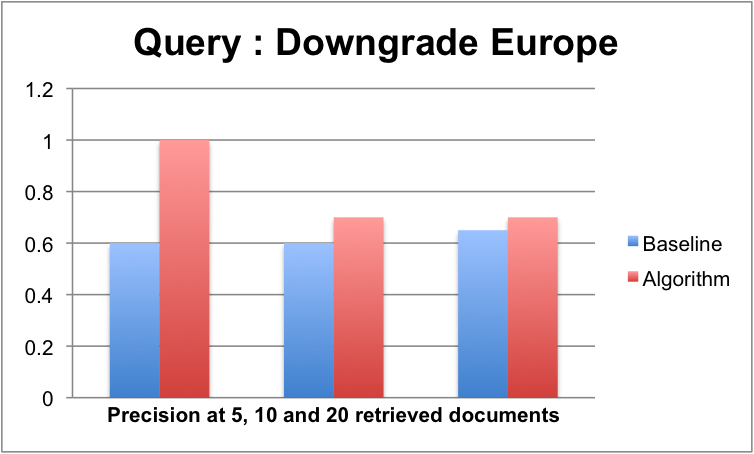
\includegraphics[scale=1.00]{downgrade_Europe.png}
\end{center}

\begin{center}
	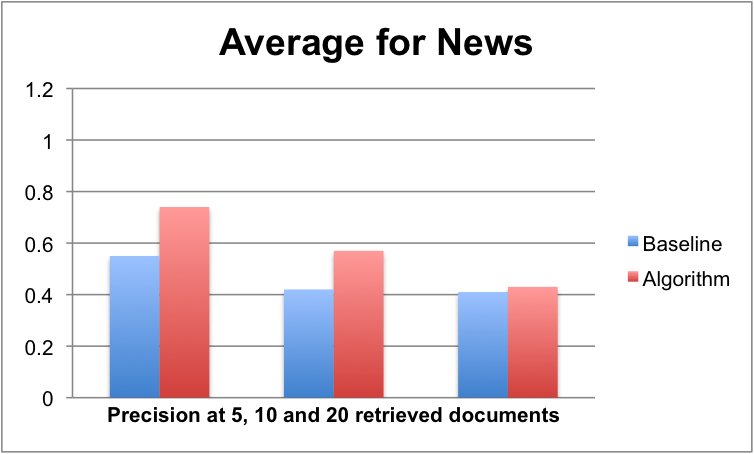
\includegraphics[scale=1.00]{Average_News.png}
\end{center}


%In order to evaluate the system, we have decided to compare it to a baseline. Like said before, the baseline is a round robin ranking based on the ranking provided by the different APIs.

%To determine if a document is relevant or not, we need the users to say it. Thats why we published a test version of our system online. This version was providing 2 sets of results for a query. The first set was the baseline and the second was our ranked results. The user had the possibility to say for each result if it was relevant or not. The results were then sent to us by email and we were able to compare the different precision (P@5, P@10 and P@20)

%-------------------------------------------%
\section{Discussion and Conclusions}
%-------------------------------------------%

\subsection{Discussions about the system}

During the use of Twitter in the algorithm, when finding interesting words, the first words found can be "obvious" and therefore not meaningful for the currents topics about the query. For example when the user search for "Obama", the first two words being returns are "president" and "barrack" so results with these words will have a higher score. But it's not giving any information about the news related to "Obama". So it's better if the user enter "president barrack obama" as a query, the results are improved in this case.

\subsection{Difficulties encountered}

\paragraph{Lack of possibilities for Google News}Because there is no API provided for Google News, we had to use an RSS feed. But this RSS feed lack in information about the documents. For example, we can't have information about the number of views of a news like for YouTube or Flickr.

\paragraph{Lack of information in a Flickr image}With Flickr, most of the images don't have any descriptions and sometimes, the title is not very explicit. So it was really difficult to find appropriate content using this source. Maybe it would be better to use another source better suited for this kind of search. 

\paragraph{Twitter links}As we have seen in our algorithm we used Twitter links to rank the documents. However, most of the links published using Twitter are shortened and therefore it is impossible to know where this link is leading. We could have found the real link behind the shortened ones but it would have took too much time and the results would not have been given to the user in an acceptable time.

\paragraph{The system is slow}Our system is for the moment a little bit slow and take around 10seconds to deliver the newspaper. As everybody is used to have instant search like on Google, Yahoo or Bing, it is hardly acceptable. Probably some optimizations in the code could have been made to solve this issue.


%\newpage
%\bibliographystyle{plain}
%\bibliography{biblio}


\end{document}

